
\chapter{Phasing very large samples}

SHAPEIT2 was initially published with the goal of phasing unrelated samples of individuals, and was shown to be the most accurate method for this task in its original paper. In the previous chapter we demonstrated that SHAPEIT2 is in fact the most accurate method over a surprisingly large range of demographic scenarios.  Whilst computationally tractable, SHAPEIT2 is not the fastest algorithm available.  On the samples analysed in the previous chapter, both HAPI-UR and Beagle were substantially faster.  Running times on chromosome 10 for each cohort are shown in figure~\ref{fig:timing-summary}.  We argue that for these sample sizes a factor of $\approx5$ in computation time is not a large sacrifice to make for the accuracy gains of SHAPEIT2.  Additionally SHAPEIT2 has a very convenient multi-threading functionality which means end-users can exploit multi-core systems with ease, hence the computational cost is largely mitigated for these ranges of $N$.

However, the age of $N>~$100,000 is upon us. For example the UK Biobank intends to genotype 500,000 individuals on Affymetrix Axiom microarrays\footnote{\url{http://www.ukbiobank.ac.uk/about-biobank-uk/}} and 100,000 individuals were recently assayed in Kaiser Permanente's Research Program on Genes, Environment and Health\footnote{{\url{http://www.rpgeh.kaiser.org/}}}. Phasing and imputation will be necessary to fully exploit such data sets and hence computationally tractable software for these tasks is needed.

\begin{SCfigure}
  \centering
  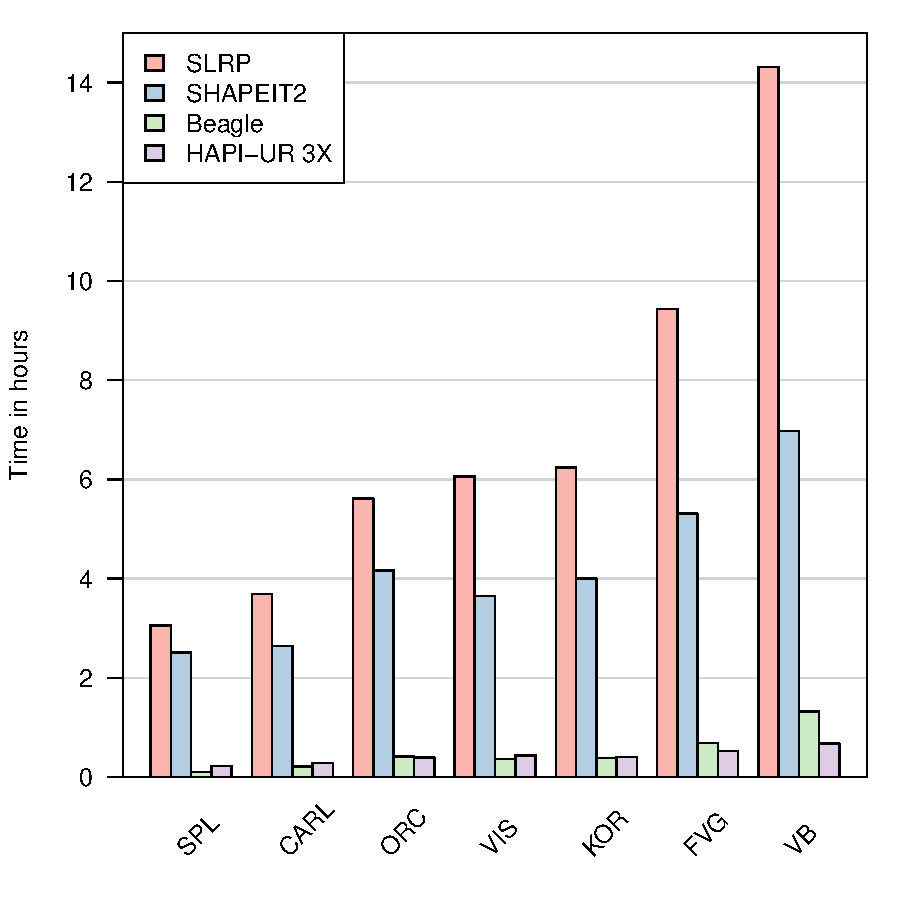
\includegraphics[width=.5\textwidth]{chap4figs/timingsummary}    
  \caption[Summary of phasing computation for isolates cohorts]{Computation time in hours for phasing chromosome 10 for each of the full cohorts described in Chapter 4.  All jobs were run on an Intel Xeon CPU E5-2690 (2.90GHz) CPU with 256GB of RAM.  Whilst no parallelism was employed here, options exists for exploiting multiple processors with varying degrees of difficulty for each piece of software.  \label{fig:timing-summary}}
%SHAPEIT2 and SLRP have the ability to run on $N$ threads resulting in an approximately $N \times$ reduction in computation time.  HAPI-UR  can be run as three simultaneous processes rather than sequentially.  Most simply, the genome can be partitioned into chunks which are phased separately with the results being ligated.
\end{SCfigure}
\newpage
In this chapter we concern ourselves with the scalability of different algorithms.  For $N=1,000$ all algorithms mentioned in the previous chapter will run within one day on a modern server with multiple CPUs, but when $N>>10,000$ the computational costs of phasing become a serious concern.  None of the techniques described in this thesis scale linearly with sample size, so na\"{\i}vely extrapolating from figure~\ref{fig:timing-summary} would be foolish.  SHAPEIT2's distance calculations incur a quadratic complexity term, but these are performed very rapidly with look-up tables so it was not clear when this quadratic component will begin to dominate computation. HAPI-UR and Beagle both need to build their respective haplotype graphs on each iteration which has complexity that is sub-quadratic but super-linear.  HAPI-UR's primary use-case is to phase very large samples tractably and it is currently the fastest method available as demonstrated in recent publications~\citep{williams2012phasing,delaneau2013}, although it is less accurate than SHAPEIT2.

In this chapter we evaluate the scalability and accuracy of HAPI-UR and SHAPEIT2 as sample sizes become very large.  We also introduce a further approximation to SHAPEIT2 to reduce the number distance calculations it has to perform, with the goal of making the non-HMM component of the algorithm scale linearly.  Since large data sets ($N>>10,000$) are currently not easy to obtain, we use a combination of real and simulated data for evaluation purposes.

\section{Reducing the complexity of SHAPEIT2's distance calculations}  
The current release of SHAPEIT2 selects a set of $K$ conditioning haplotypes for an individual being updated.  The set of $K$ conditioning haplotypes are denoted as  $H^{*}$ and are a subset of the  full set of haplotypes in the cohort, $H$. Computational cost and accuracy both increase with $K$, the default of $K=100$ generally gives good results. Chromosomes are divided into roughly equally size windows and  a different set of $H^{*}$ is chosen for different windows. Window size is a tuneable parameter and the default size for microarray data is 2Mb.  Conditioning haplotypes are selected for an individual being phased by taking the $K$ haplotypes in the sample with the closest Hamming distances from the individual's haplotypes from the previous iteration, say $(h^1,h^2)$. The idea being that this will yield more closely related conditioning haplotypes which are more informative of phase.

One caveat with this approach is that individuals that share a region of genome where \emph{both} haplotypes are identical-by-descent (IBD=2) are uninformative of phase and can cause the algorithm to get stuck in a poor quality solution.  Hence individuals that are  IBD=2 within a region are excluded from the set of possible conditioning haplotypes. Details of how the IBD=2 individuals are determined are described in the supplementary of \cite{delaneau2013}. 

The algorithm for selecting conditioning haplotypes is then as follows:

\vspace{10pt}
\begin{algorithm}
  \caption{SHAPEIT2 haplotype selection}
  \begin{algorithmic}[0]    
    \State Select $W\subseteq H$ such that haplotypes in $W$ are unlikely to be from IBD=2 individuals
    \ForAll{$H_j\in W$}
    \State    Calculate $D(H_j) = \textrm{min}(\textrm{\texttt{hamming}}(h^1,H_j),\textrm{\texttt{hamming}}(h^2,H_j))$
    \EndFor
    \State    Sort $W$ by ascending $D(H)$ values    
    \State \textbf{return} the first $K$ haplotypes in $W$
  \end{algorithmic}
\end{algorithm}
where $\textrm{\texttt{hamming}}(h,H)$ is the Hamming distance between the two haplotypes, that is the count of binary differences.

 If we assume that the number of haplotypes in $W$ is $M\approx2(N-1)$ then this algorithm has complexity $O(N^2L)$ which is undesirable when $N$ becomes large. However, the filtering of IBD=2 individuals suggests an obvious way of controlling complexity. If we could limit the size of $W$ to $M$ elements then the algorithm would have complexity $O(NML)$, if we could keep $M$ constant then we would have an algorithm with complexity $O(NL)$ which is our desired outcome.  Most simply, we could create $W$ by randomly sampling $M$ haplotypes, we refer to this method as SHAPEIT2-random. We evaluate such an approach as well a more sophisticated partitioning approach described next.  We refer to the set $W$ as the `candidate haplotypes'.  In all comparisons we set $M=1000$, further work will involve tuning this parameter.

\subsection{K-Means clustering to partition the data}
Given a set of haplotypes within a window, $H=\{H_1,\ldots,H_N\}$, we could assign class labels to each observation, say $C_i \in \{1, \ldots ,J\}$, such that observations with the same label are similar according to some metric. We can then assign the candidate haplotypes for each individual $i$ as $W_i = \{H_j: C_j =C_i \}$. This is a more a principled approach than choosing $W$ at random, but does require a fast clustering method.

K-Means clustering is a well known technique that minimises the within-cluster sum of squares:
$$\sum_{i=1}^N \sum_{l=1}^L (H_{il} - \mu_{C_i l})^2$$
where $\mu_C$ is the cluster mean for class $C$.  The simplest way to minimise this objective function is to iteratively assign class labels to each observation based on which cluster mean is closest and then recalculate the mean, continuing until convergence~\citep{lloyd1982least}. \cite{arthur2007k} proposed ``K-means++'' which provides an algorithm for choosing starting values that are well dispersed and tend to lead to convergence to better optima with less iterations.

We implemented K-means++ within SHAPEIT2 and applied it to all haplotypes within each window running it for 10 iterations or until convergence, 10 iterations is usually insufficient for convergence but we only require a rough partitioning.  If we want clusters of roughly size $M$ then we set the number of clusters $J=2N/M$. If we make the assumption that K-Means results in a perfectly equal partitioning then the SHAPEIT2 distance calculations will have complexity $O(NML)$. The K-Means algorithm has complexity $O(NIJ) = O(N^2I/M)$ where $I$ is the number of iterations.  Whilst this is still scaling quadratically with $N$, the divisor $M$ controls computation well for the sample sizes we investigate.  We refer to this modification as SHAPEIT2-kmeans.

A problem with this approach is that a haplotype's nearest neighbours are not guaranteed to be within the same cluster  and hence may not be identified.  This is likely to be the case  for individuals on the boundary of a cluster. Figure~\ref{chap5:kmeans} gives a toy example demonstrating this problem. 
\begin{SCfigure}[1][h]
  \centering
  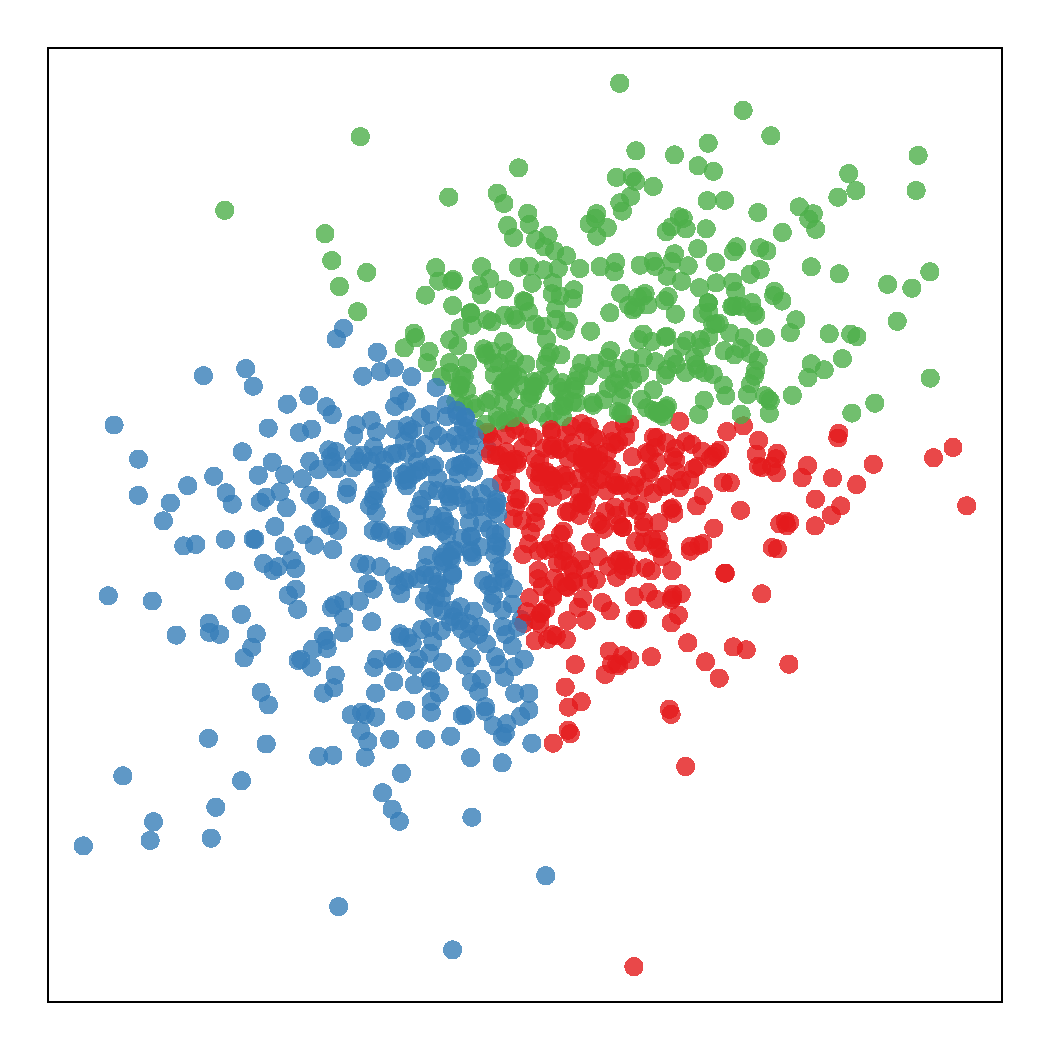
\includegraphics[width=.45\textwidth]{chap5figs/kmeans-example}
  \caption[K-Means toy example]{A toy example for K-Means on some simulated bivariate data with three clusters coloured red, green and blue.  Whilst  an observation's nearest neighbours are usually within the same cluster, points on the boundary will have nearest neighbours in a different cluster.  If we only search for nearest neighbours within the same cluster, the solution will be sub-optimal. This data is simulated on from a bivariate normal distribution which is obviously different to the haplotype data we work with, but the same principal applies.\label{chap5:kmeans}}
\end{SCfigure}

%% \subsection{Partitioning on the first principal component}
%% Principal Component Analysis (PCA) is a popular method for dimension reduction and has proved to be an extremely powerful took in genetics for quantifying broad scale relatedness between individuals using genotype data~\citep{patterson2006population,novembre2008genes,mcvean2009genealogical}.  The engine underlying PCA is the singular value decomposition (SVD) of a design matrix $X$:
%% $$\textbf{X} = \textbf{U} \textbf{D} \textbf{V}^T $$
%% here $X$ is our haplotype data with $2N$ rows and $L$ columns.  The columns of $\textbf{U} \textbf{D}$ are the principal components (PC1,PC2,...,PC$L$) of $\textbf{X}$ where the PC1 is the linear combination of genotypes with the maximum variances, PC2 is orthogonal to PC1 and has the maximum remaining variance and so forth. 

%% The SVD has complexity $O(N^2L)$ when $N>L$ (which is likely the case here), but if we have the matrix $\textbf{V}$ we can rotate $\textbf{X}$ accordingly to find the PCs.  We simply sub-sample one thousand rows of $\textbf{X}$ to calculate an approximate  $\textbf{V}$ and then rotate the full  $\textbf{X}$, finding approximate principal components constraining the SVD computation to $O(L)$. Let $\textrm{PC1}_i$ be the first principal component for haplotype $H_i$. We then choose $W_j = \{H_j : |\textrm{PC1}_i-\textrm{PC1}_j| < q_{M/2}\}$ where $q_{M}$ is the $M/(2N)$th quantile of all differences from $\textrm{PC1}_i$. That is, we find the $M$ closest values on the first principal component, these can be found with $O(M)$ complexity by storing the PC1s has a sorted list and using a binary search~\citep{skiena1998algorithm}.

%% Reducing a haplotype with hundreds of SNPs to one dimension is likely to result in a substantial loss of information so this approach is very approximate.  However the described algorithm is very fast and may prove superior to the randomised approach.

\section{Data}
\subsection{Real data}
We merged all the cases and controls from the Wellcome Trust Case Control Consortium 1~\citep{consortium2007} (WTCCC1) along with the 60 European individuals taken from the parents of 90 mother-father-child trios available from the HapMap cohorts~\citep{hapmap2}.  The parents from the trios provide us with true underlying haplotypes for individuals of similar ethnicity to those individuals in the WTCCC1 cohort.  The WTCCC1 individuals were assayed on the Affymetrix 500K genotype microarray and the HapMap individual's SNPs were filtered to match the markers on this chip.  This provides us with a sample of $N=16239$ with 60 validation individuals. We analysed 10Mb of data from chromosome 10 in these experiments (60Mb-70Mb).

\subsection{Simulated data}
We simulated genetic variants across 10Mb of DNA for 100,000 haplotypes, to create 50,000 diploid individuals. Simulations were performed using the Markovian Coalescent Simulator (MaCS) software~\citep{chen2009fast} which allows approximate simulation from the coalescent for genomic sequences up to the length of whole chromosomes with arbitrary demographic histories.  We used the demographic model specified by \cite{schaffner2005calibrating} whom calibrated the model to empirical measures of linkage-disequilibrium and the variant frequency spectrum observed in real data.  The combined genetic map from the HapMap project~\citep{hapmap2} for chromosome 1 (63Mb - 73Mb) was supplied to MaCS for simulations.  Finally we sampled variants from this simulated data in a stratified manner giving similar physical spacing between SNPs and  allele frequency spectrum to the Affymetrix 500K chip that was used on the WTCCC1 cohort described previously.  Genotyping error was introduced in the same way as described in the chapter 4 simulation experiments.

\section{Results}
We randomly sampled subsets of differing size on both the real and simulated data to evaluate how the accuracy and computation scales with sample size for each method.

\subsection{Profiling}
We first profiled the computation of the standard implementation of SHAPEIT2 on our simulated data.  Figure~\ref{chap5:s2-profile} shows what proportion of time SHAPEIT2 spends on each of its computational components as $N$ increases.  For small sample sizes the HMM component of the model completely dominates computation.  Once sample sizes increase past 10,000 the distance calculations begin to account for a substantial amount of the computation time.  For N=50,000 we estimate SHAPEIT2 would take 377.7 days to phase the whole genome (although this task would be easily parallelised), 83.6\% of this computation time would involve distance calculations.  
\begin{SCfigure}[1][h]
  \centering
  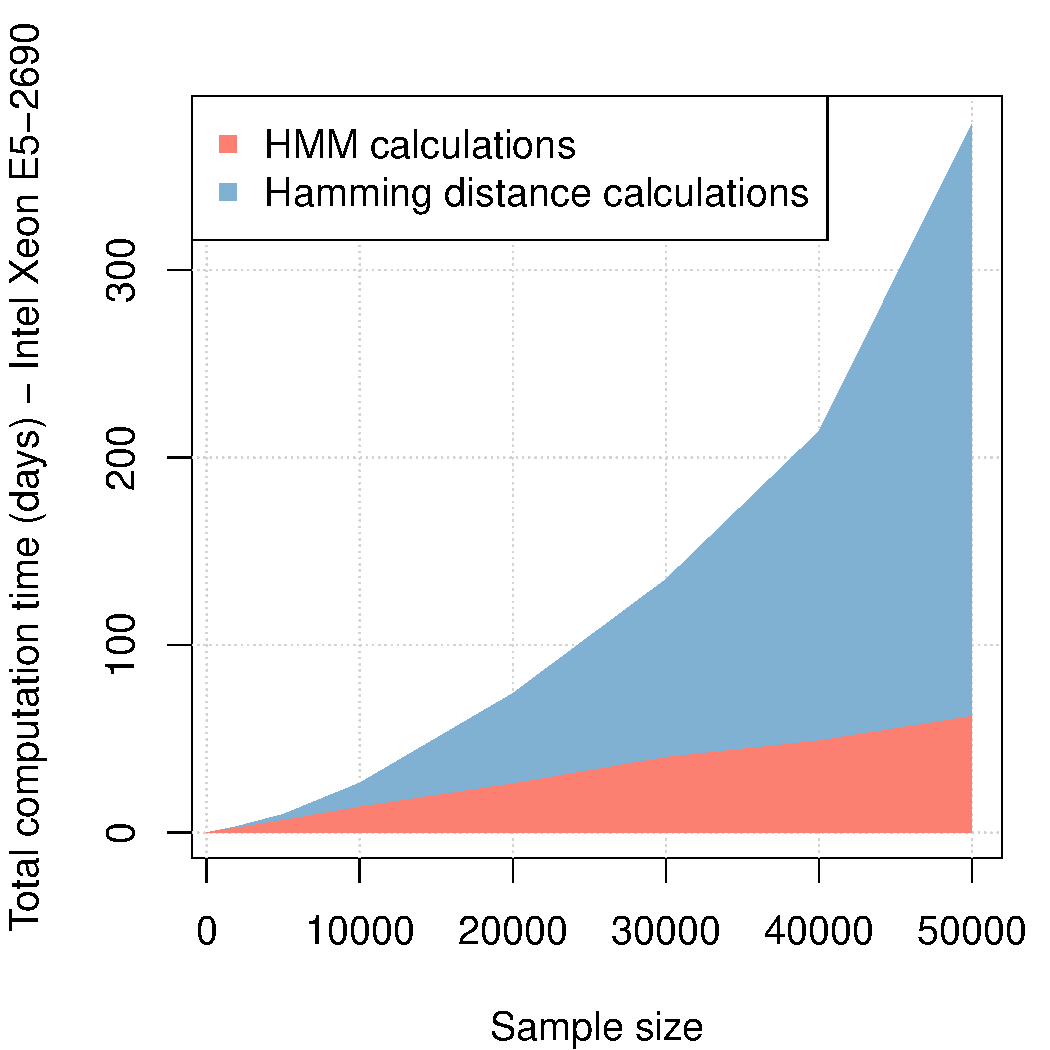
\includegraphics[width=.5\textwidth]{chap5figs/shapeit2_profiling}
  \caption[SHAPEIT computation profiling]{Profiling of the standard version SHAPEIT2's computational load on our simulated data set for increasing values of $N$. Computation time is in days (extrapolated from computations on a 10Mb region).  The blue area is the time spent on Hamming distance calculations. The light red area is the time spent on all other computations. The height of the curve is total computation time. When $N>10000$ the Hamming distance calculations rapidly begin to dominate computation. \label{chap5:s2-profile}}
\end{SCfigure}

\subsection{Performance on real data}
Figure~\ref{chap5:switch} (top) plots the switch error rate (left) and computation time in days (right) for varying sample sizes on the HapMap+WTCCC1 data. Switch error rates for N=1,000 were  2.1\%, 2.0\%, 2.15\% and 2.9\% for SHAPEIT2, SHAPEIT2-Random, SHAPEIT2-kmeans and HAPI-UR respectively which is in line with previously published results. It is interesting the random approach does marginally better here but this could just be due to the fact SHAPEIT2 is using stochastic algorithm to estimate haplotypes. Switch error for SHAPEIT2, SHAPEIT2-kmeans and HAPI-UR improve substantially as sample size increases with switch error rates of 1.28\%, 1.42\% and 1.66\% for the largest sample size of N=16,239.   SHAPEIT2-random has an error rate of 1.84\% at this sample size and appears to be beginning to plateau. SHAPEIT2-kmeans has consistently $\approx$ $0.1\%$ higher switch error than SHAPEIT2 but is still consistently more accurate than HAPI-UR.   For N=16,239, SHAPEIT2-kmeans and HAPI-UR are about 1.5 and 1.6 times faster than SHAPEIT2.  SHAPEIT2-kmeans and SHAPEIT2-random appear to be scaling linearly across this range of $N$ whilst HAPI-UR and SHAPEIT2 show greater than linear scaling.

\subsection{Performance on simulated data}
The accuracy on the simulated data is somewhat higher than what we observe on the real data sets.  At N=1,000 SHAPEIT2, SHAPEIT2-random, SHAPEIT2-kmeans and HAPI-UR  have switch error rates of 3.66\%, 3.77\%, 3.62\% and 8.79\% respectively, decreasing to  0.47\%,  3.25\%, 0.629\%  and  0.85\% for N=50,0000. The random selection method sees little improvement in accuracy after N=10,000 in this data.  SHAPEIT2 remains the most accurate method across the range of sample sizes, followed by SHAPEIT2-kmeans and then HAPI-UR.

The more interesting results are the computation times.  SHAPEIT2-kmeans scales linearly across this range of $N$ whilst the super-linear scaling of HAPI-UR  means it is slightly slower than SHAPEIT2-kmeans at N=50,000.  SHAPEIT2-kmeans is 4.57 times faster than SHAPEIT2 and 1.08 times faster than HAPI-UR  at N=50,000.  The K-means approach is also faster than SHAPEIT2-random despite having greater theoretical complexity.  This is because we put considerable effort into optimising the K-means clustering routine whilst the random generation of candidate haplotypes was implemented with a simplistic rejection sampling scheme. 

\begin{figure}
\centering
\textbf{WTCCC1 + HapMap Data}\\
   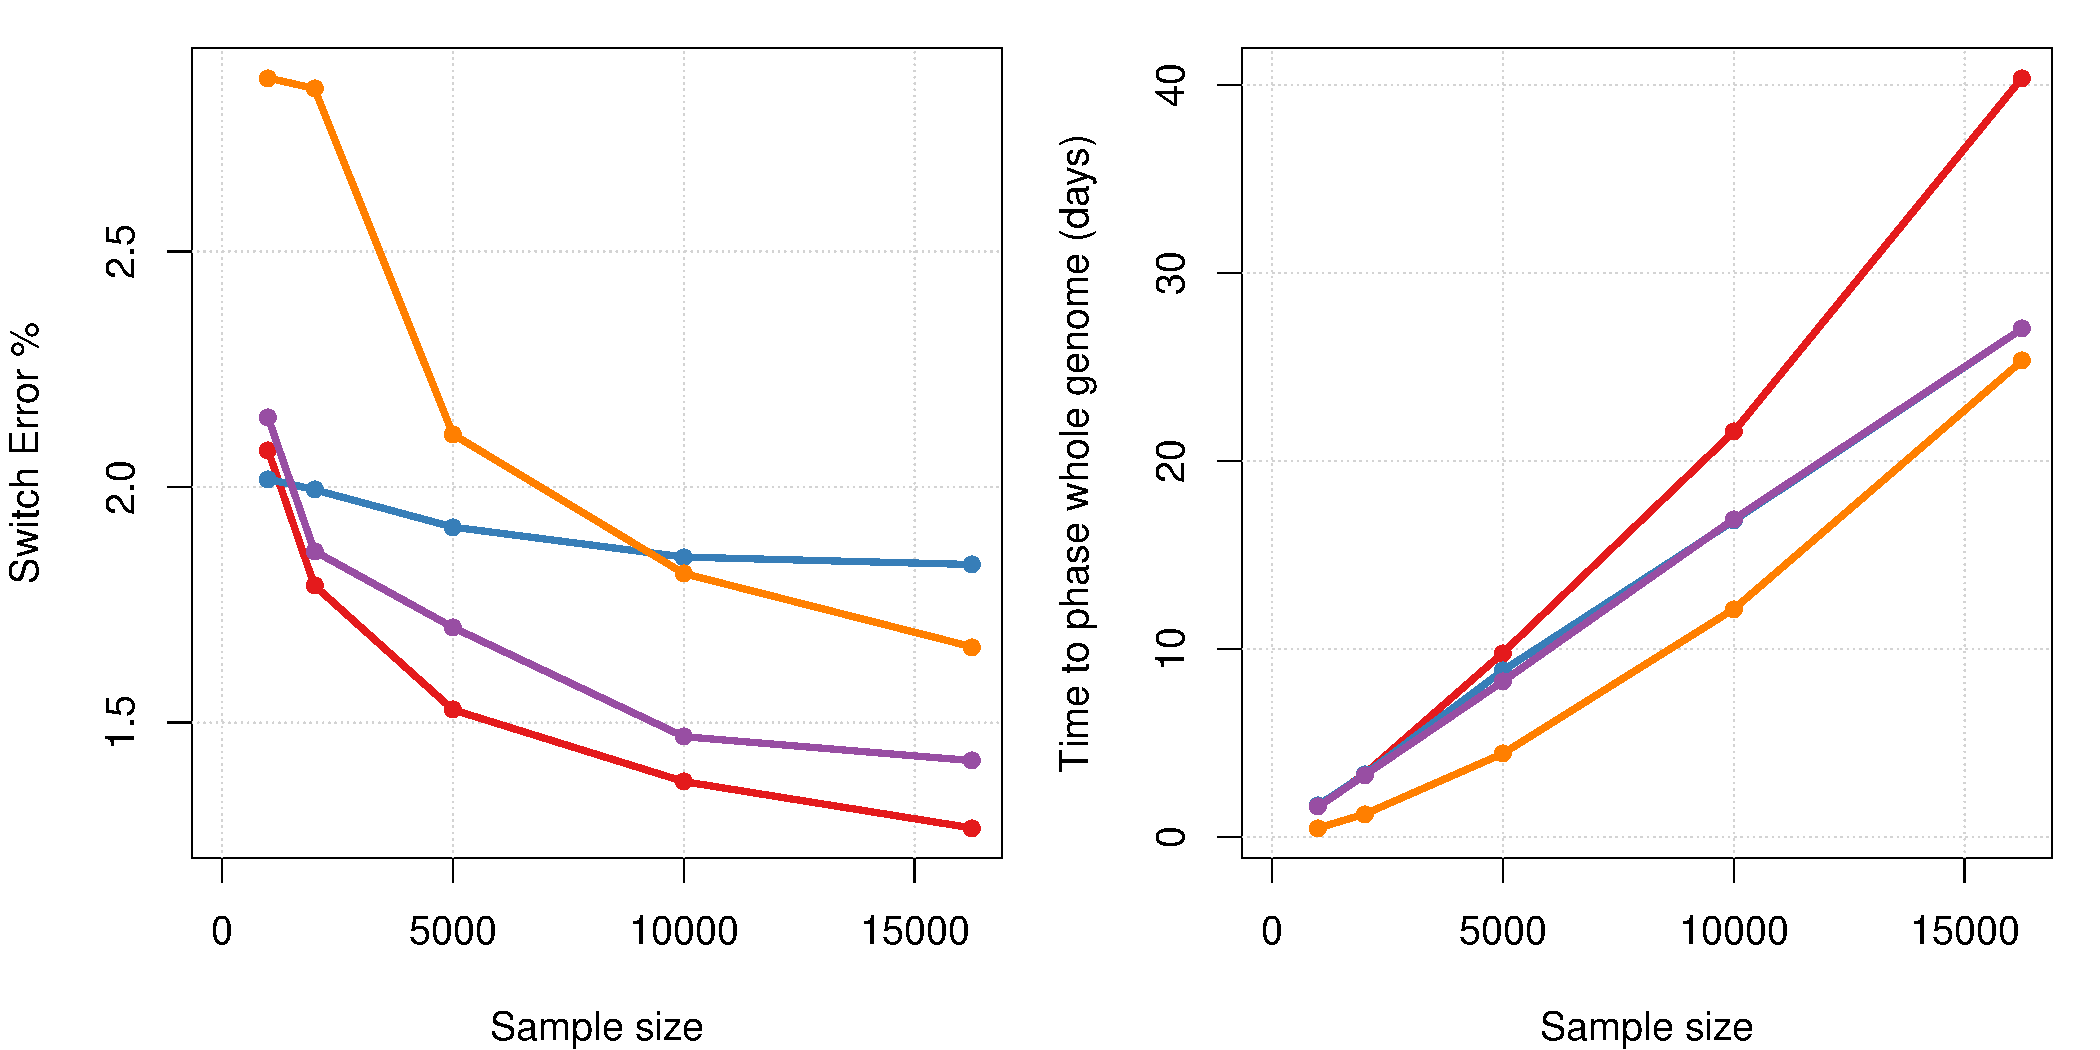
\includegraphics[width=\textwidth]{chap5figs/wtccc}\\%\vspace{-20pt}\\
\vspace{20pt}
\textbf{Simulated data}\\
   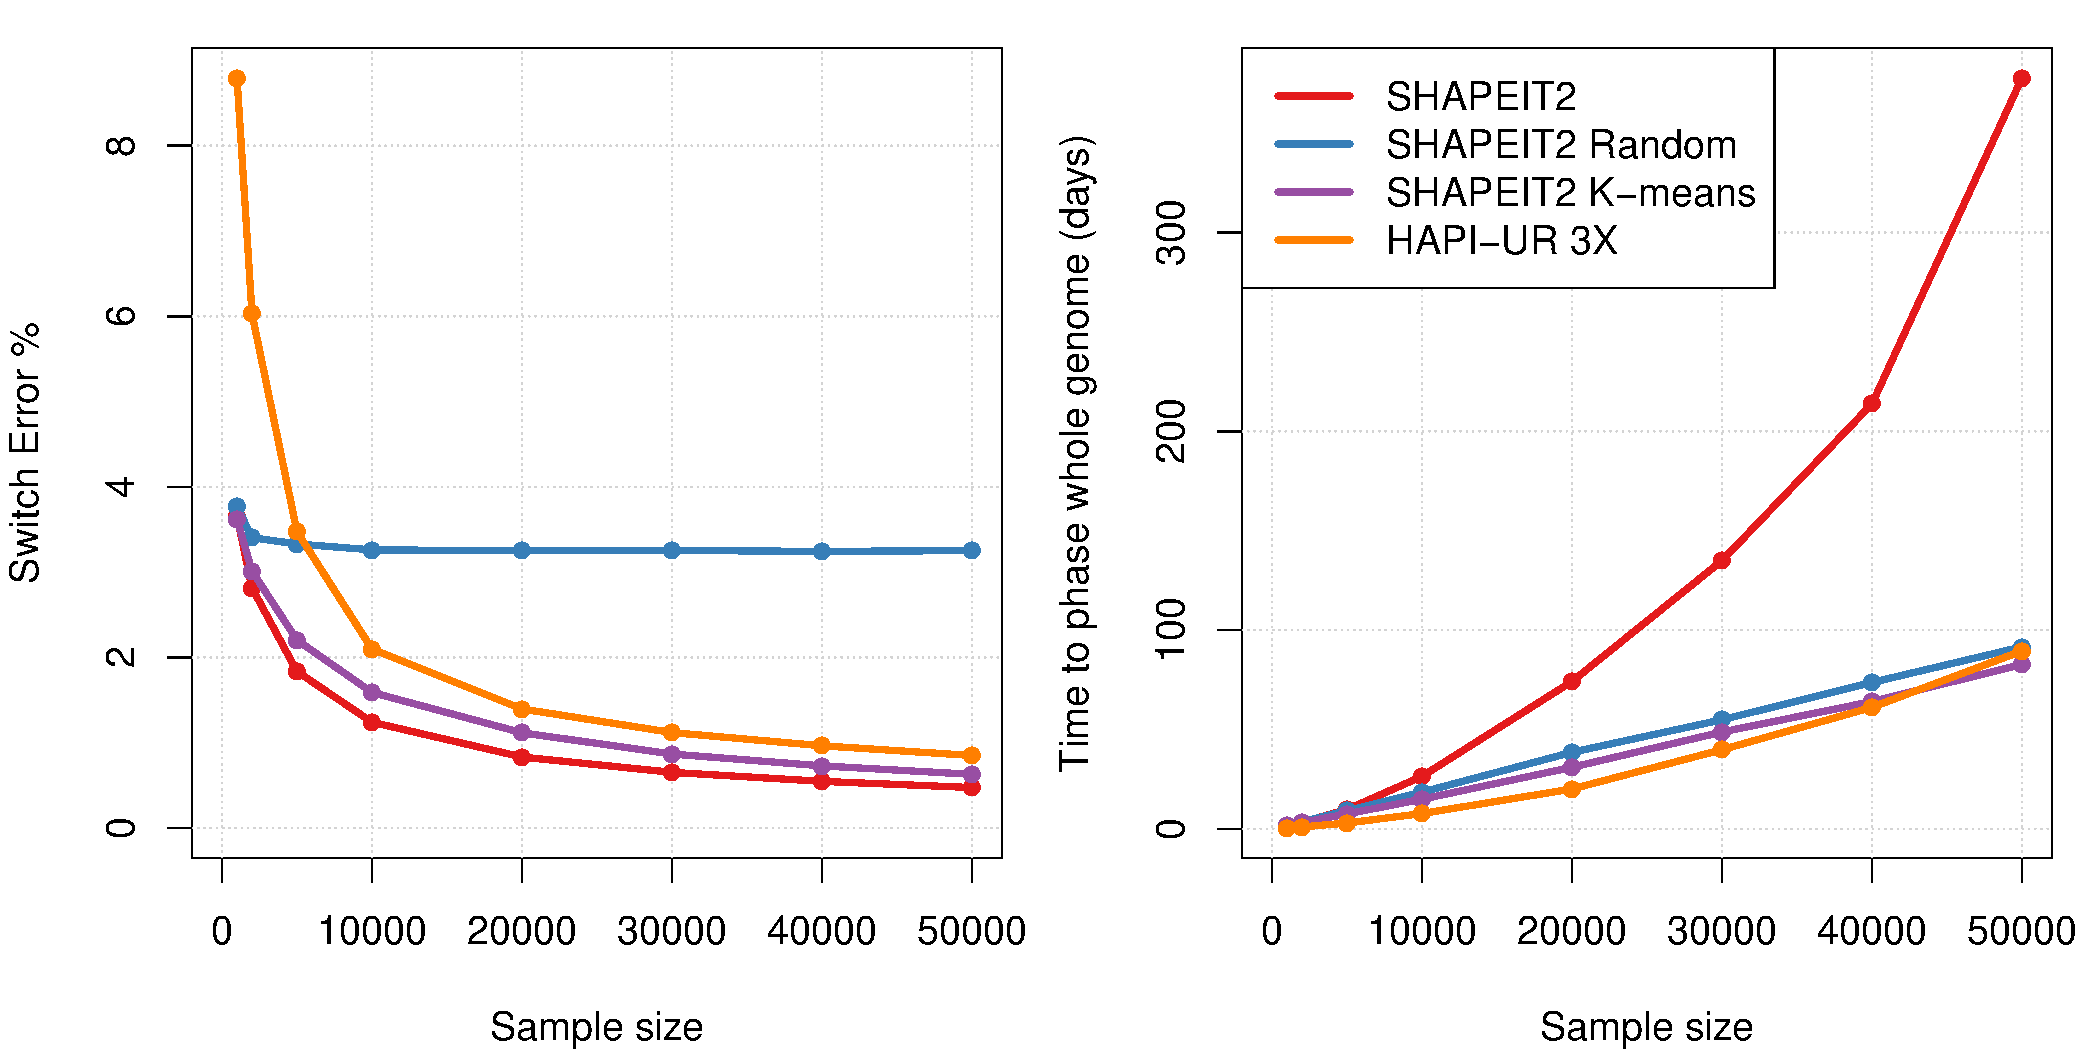
\includegraphics[width=\textwidth]{chap5figs/simulated}%\vspace{-20pt}
\caption[Accuracy and computation comparison for increasing sample sizes]{Accuracy and computational cost of different phasing routines on the WTCCC1+HapMap data (top) and the simulated Affymetrix 500 data (bottom). SHAPEIT2 is the standard implementation with a quadratic distance cost, `Random' does distance calculations on $M$ randomly chosen haplotypes, `K-means' compares all individuals within the same cluster resulting $\approx M$ comparisons per individual. We used $M=1000$ in all cases.  HAPI-UR3X  is three averaged runs of HAPI-UR. \textbf{Left:}~The switch error rate against sample size.  \textbf{Right:} The single CPU computation time in days for whole genome phasing (extrapolated from 10Mb) for each method on an Intel Xeon CPU E5-2690 (2.90GHz) CPU with 256GB of RAM. \label{chap5:switch}}
\end{figure}

\section{Discussion and Further Work}

The methods and results in this chapter are very preliminary, but are proof of the concept that SHAPEIT2 can be extended to larger samples. We saw that the K-means approach was quite effective at controlling computation whilst maintaining accuracy, resulting in a method that was more accurate and faster than HAPI-UR at 50,000 samples.  We hope to remove the modest loss of accuracy introduced with further modifications to the K-means partitioning technique. We also need to investigate how to correctly set the value of $M$.

The loss of accuracy when using K-means is likely due to the fact that a haplotype's nearest neighbour is not always in the same cluster, particularly for haplotypes that lie on the boundary between clusters.  A possible workaround to this problem would be to  allow observations to lie in multiple clusters, this is a similar idea to ``Canopy Clustering'' which is a popular method in data mining communities~\citep{mccallum2000efficient} for rapidly clustering large high-dimensional data sets. 

We have restricted our evaluations to using the Hamming distance metric, but there is no reason a more sophisticated distance measure could not be used.  One obvious measure would be to use the Euclidean distance between normalised alleles, $x_{il} = \frac{(H_{il} - p_l)}{\sqrt{p_l(1-p_l)}}$, where $p_l$ is the MAF at site $l$.  This would put greater weight on low frequency variants, which is sensible as they correlate with longer shared haplotype length.  This measure still ignores correlation between variants, we could also use the Mahalanobis distance measure which would involve modelling all SNPs in a window jointly with a multivariate normal distribution, providing a simple way of taking into LD into account.

This chapter touches on one small aspect of the issue that data is growing faster than computing power in the field of genetics.  This means that new approximate (but accurate) algorithms constantly need to be developed to allow tractable computation. This trend is abundantly clear in the field of haplotype phasing where the real benefit of new methods such as SHAPEIT2 and HAPI-UR has not only been improved accuracy, but substantially decreased computation time.
